% !TeX encoding = UTF-8
% !TeX root = MAIN.tex

\ifeng 
	\chapter*{Statutory Declaration}
	I hereby declare that the thesis submitted is my own unaided work, that I have not used other than the sources indicated, and that all direct and indirect sources are acknowledged as references.

	This printed thesis is identical with the electronic version submitted.

	\vskip2cm
                          
	\place, \date       \hspace*{0pt}\hfill   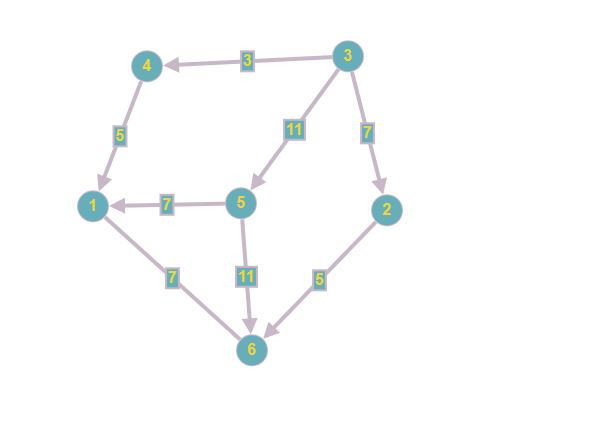
\includegraphics[width=6cm]{pics/divs/sign.JPG}



\else 
	\chapter*{Eidesstattliche Erklärung}
	Ich erkläre an Eides statt, dass ich die vorliegende \ifcase\type Arbeit \or Bachelorarbeit \or Masterarbeit \or Dissertation \or Diplomarbeit \fi selbstständig und ohne fremde Hilfe verfasst, andere als die angegebenen Quellen und Hilfsmittel nicht benutzt bzw. die wörtlich oder sinngemäß entnommenen Stellen als solche kenntlich gemacht habe.

	Die vorliegende \ifcase\type Arbeit \or Bachelorarbeit \or Masterarbeit \or Dissertation \or Diplomarbeit \fi ist mit dem elektronisch übermittelten Textdokument identisch.

	\vskip1cm
	\place, \date
\fi


\ifeng
	\chapter*{Abstract}
\else
	\chapter*{Kurzfassung}
\fi

%% Hier Abstact in der Sprache eingeben, in der die Arbeit geschrieben wurde.
%% Enter here the abstract in the main language.
In recent years the use of digital learning systems boosted rapidly. The COVID-19 pandemic led to an increase of homeschooling situations, and therefore the usage of digital technology in education\cite{Alabdulaziz}. The aim of this thesis is to develop an interactive online learning software for teaching graph theory in computer science education. Graph theory has major applications in our daily life. For example, it is used in modern navigation systems to find the shortest path to the desired destination. Computer science education should be used to teach the concepts behind new technologies. The VizGraph application follows the COOL (Computer-supported Open Learning) informatics principle\cite{SabitzerCoolinfo}\cite{SabitzerCool}. VizGraph allows students to discover graph theory interactively by drawing their own graphs. It’s a modern single page web application (SPA) to draw graphs and automatically computes and visualize properties of a graph. The use of VizGraph should encourage computational thinking and solution based learning.\\ 
The application is implemented in Typescript\cite{bierman2014understanding} and uses the modern Angular\cite{jain2014angularjs} web framework. The visualization is realized with the d3.js\cite{d3js} JavaScript library. D3.js is used to generate dynamic and interactive visualizations. The main component of the web application is a graphic editor, which is structured according to the Model-View-Controller(MVC) design pattern and applies the object-oriented (OO) programming paradigm\cite{mossenbock}.\\ 
The VizGraph application allows students to easily draw their own graphs by adding nodes and edges. The app includes the following features:
\begin{itemize}
\item add nodes (vertice)
\item add connection between nodes (edge)
\item connection can be directed or undirected with weight
\item compute adjacency matrix
\item compute incidence matrix
\item compute distance matrix 
\item find shortest path (Dijkstra algorithm)
\item find cycle
\end{itemize}
It is possible to export the graph visualization as an image or to save the graph in GeoJSON\cite{rfc7946} open standard format.
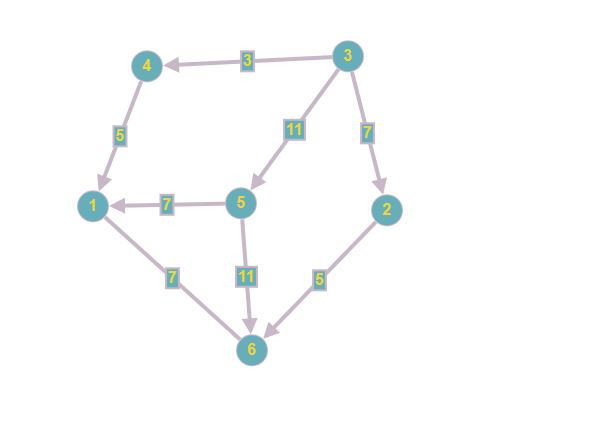
\includegraphics[width=10cm]{pics/graphen.JPG}
{
	\let\clearpage\relax
	\ifeng
		\selectlanguage{ngerman} 
		\chapter*{Kurzfassung}
	\else
		\selectlanguage{english} 
		\chapter*{Abstract}
	\fi

	%% Hier Abstact in der jeweils anderen Sprache eingeben.
	%% Enter here the abtract in the other language.
In den letzten Jahren hat sich der digitale Unterricht und die Verwendung von digitalen Lernsystemen enorm gesteigert. Die COVID-19 Pandemie f\"uhrte zu vermehrtem Homeschooling, und den damit verbundenen Einsatz von digitalen Technologien im Unterricht\cite{Alabdulaziz}. Ziel dieser Diplomarbeit ist die Entwicklung einer interaktiven online Anwendung um Graphentheorie im Informatikunterricht vorzustellen. In unserem Alltag benutzen wir oft unbewusst die Algorithmen der Graphentheorie. In modernen Navigationssystemen wird mit Hilfe der Graphentheorie der kürzste Weg zwischen zwei Orten bestimmt. Der Informatikunterricht soll nicht nur die Anwendung, sondern auch die technischen Konzepte dieser neuen Technologien vermitteln. Die VizGraph Anwendung unterst\"utzt die Sch\"uler beim Lernen nach dem COOL (Computer-supported Open Learning) Informatik Ansatz\cite{SabitzerCoolinfo}\cite{SabitzerCool}. Dabei sollen Sch\"uler spielerisch die Konzepte der Graphentheorie entdecken. Die Software ist eine moderne Single Page Web Application (SPA) und erm\"oglicht die Visualisierung von Graphen, und berechnet automatisch deren Eigenschaften. Durch das Anwenden der App soll das l\"osungsorientierte und informatische Denken der Sch\"uler best\"arkt werden.\\
Die Webanwendung ist in Typescript\cite{bierman2014understanding} programmiert, und verwendet das moderne Angular\cite{jain2014angularjs} Webframework. Die Visualisierung ist mit Hilfe der d3.js\cite{d3js} JavaScript Bibliothek umgesetzt. D3.js wird f\"ur die Erzeugung von dynamischen interaktiven Grafiken verwendet. Die Hauptkomponente der  Webanwendung ist ein Grafikeditor zum Zeichnen des Graphen. Dieser basiert auf dem Model-View-Controller(MVC) Entwurfsmuster und ist objektorientiert(OO) programmiert\cite{mossenbock}.\\ 
Die VizGraph Webanwendung bietet den Sch\"ulern eigene Graphen zu zeichnen, indem sie Knoten und Kanten einfach hinzuf\"ugen. Die Anwendung beinhaltet die folgenden Funktionalit\"aten:
\begin{itemize}
\item Knoten hinzuf\"ugen
\item Kante hinzuf\"ugen
\item gerichtete oder ungerichtete Kanten mit Gewicht
\item Bestimmten Adjazenzmatrix
\item Bestimmten Inzidenzmatrix
\item Bestimmten Distanzmatrix 
\item K\"urzesten Pfad bestimmen (Dijkstra Algorithmus)
\item Kreisfreite Graphen
\end{itemize}
Die Graphen k\"onnen entweder in einer Bilddatei, oder im GeoJSON\cite{rfc7946} offenen Standardformat abgespeichert werden.
	\ifeng
		\selectlanguage{english}
	\else
		\selectlanguage{ngerman}
	\fi
}
